% slides.tex
\documentclass[20pt]{beamer}
\usepackage{listings}
\usepackage[utf8]{inputenc}
\usepackage{color}
\usepackage{graphicx}

\usetheme{default}
\usecolortheme{dove}
\useoutertheme{default}

% Slightly smaller title
\setbeamerfont{frametitle}{size=\large}
\setbeamerfont{verb}{size=\small}

% lst settings
\lstset{
    language=Haskell,
    basicstyle=\small,
    gobble=4
}

\newcommand{\vspaced}{
    \vspace{5mm}
}

\begin{document}

\title{Laziness}
\subtitle{BarcampGhent 4}
\author{Jasper Van der Jeugt}
\date{May 25, 2011}

\begin{frame}[plain]
    \titlepage
\end{frame}

% Introduction
% ------------

\begin{frame}{Hello!}
    My name is Jasper \\
    Student at UGent \\
    I write Haskell \\
    GhentFPG \\
    \texttt{@jaspervdj} \\
    \texttt{jaspervdj.be}
    \begin{picture}(0.0, 0.0)
    \put(40.0, -15.0){
        
\includegraphics[width=0.5\textwidth]{../2011-functionalpx-blaze-html/images/hat.pdf}}
    \end{picture}
\end{frame}

\begin{frame}{Overview}
    \textbf{Introduction} \\
    What is laziness? \\
    Lazy lists \\
    Composability \\
    Lazy I/O \\
    (Examples)
\end{frame}

% What is laziness?
% -----------------

\begin{frame}{Overview}
    Introduction \\
    \textbf{What is laziness?} \\
    Lazy lists \\
    Composability \\
    Lazy I/O \\
    (Examples)
\end{frame}

\begin{frame}{What is laziness?}
    \textit{A procastrinating runtime}
\end{frame}

\begin{frame}[plain]
    \begin{center}
    
\includegraphics[height=0.9\textheight]{images/reddit.pdf}
    \end{center}
\end{frame}

\begin{frame}{What is laziness?}
    \textit{When do you think \newline these slides were made?}
\end{frame}

\begin{frame}{What is laziness?}
    \textit{Laziness for programming languages?}
\end{frame}

\begin{frame}[plain]
    \begin{center}
    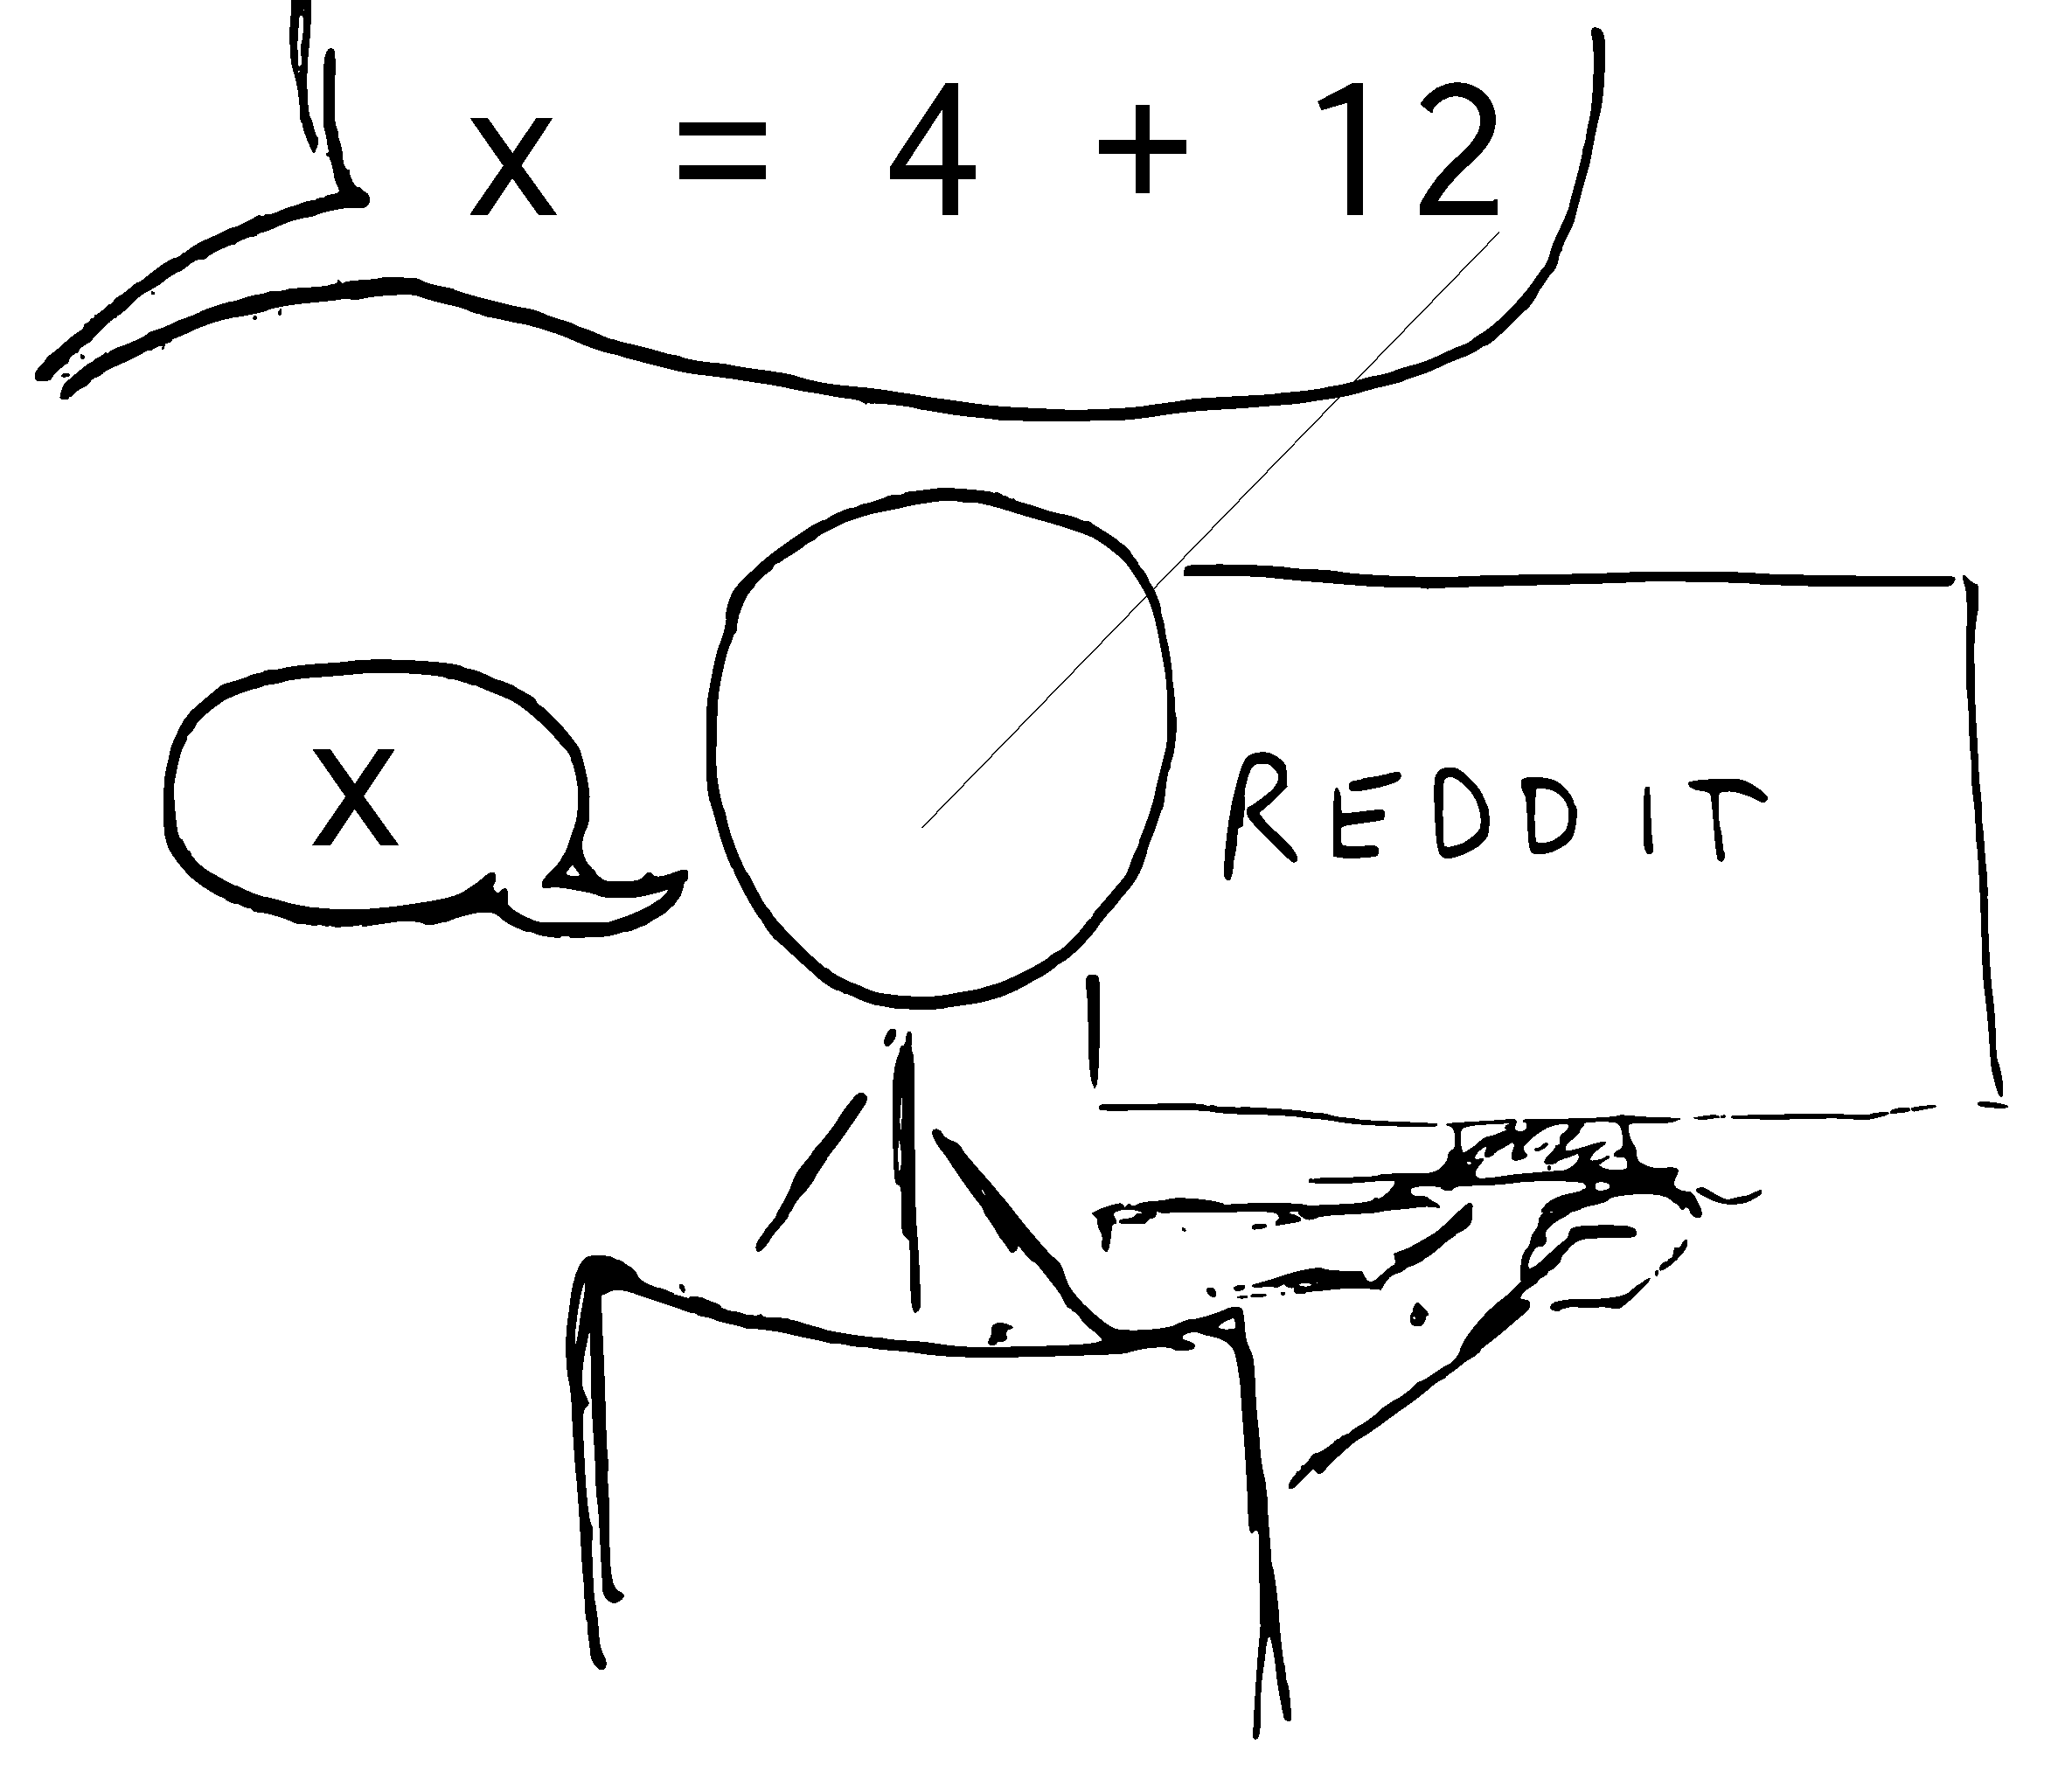
\includegraphics[height=0.9\textheight]{images/reddit-binding.pdf}
    \end{center}
\end{frame}

\begin{frame}[plain]
    \begin{center}
    
\includegraphics[height=0.9\textheight]{images/reddit-eval.pdf}
    \end{center}
\end{frame}

\begin{frame}{What is laziness?}
    This sounds like a pretty stupid idea
\end{frame}

\begin{frame}{What is laziness?}
    But actually it is \textit{very} powerful
\end{frame}

% Lazy lists
% ----------

\begin{frame}{Overview}
    Introduction \\
    What is laziness? \\
    \textbf{Lazy lists} \\
    Composability \\
    Lazy I/O \\
    (Examples)
\end{frame}

\begin{frame}{Lazy lists}
    A list of all primes? \\
    A list of all even numbers?
\end{frame}

\begin{frame}[fragile]{Lazy lists}
    \begin{lstlisting}
    ones = 1 : ones
    \end{lstlisting}
\end{frame}

\begin{frame}[fragile]{Lazy lists}
    \begin{lstlisting}
    evens = filter even [1 ..]
    \end{lstlisting}
\end{frame}

\begin{frame}[fragile]{Lazy lists}
    \begin{lstlisting}
    fibs = 1 : 1 :
        zipWith (+) fibs (tail fibs)
    \end{lstlisting}
\end{frame}

% Composability
% -------------

\begin{frame}{Overview}
    Introduction \\
    What is laziness? \\
    Lazy lists \\
    \textbf{Composability} \\
    Lazy I/O \\
    (Examples)
\end{frame}

\begin{frame}{Composability}
    Lazy functions are more composable and allow more code reuse
\end{frame}

\begin{frame}[fragile]{Composability}
    \begin{lstlisting}
    any odd [2, 4, 7, 10]
    \end{lstlisting}
\end{frame}

\begin{frame}[fragile]{Composability}
    \begin{lstlisting}
    any f list = or (map f list)
    \end{lstlisting}
\end{frame}

\begin{frame}[fragile]{Composability}
    \begin{lstlisting}
    any f list = or (map f list)
    \end{lstlisting}
    \vspaced
    Imagine an expensive \texttt{f}. Will we short-circuit?
\end{frame}

\begin{frame}[fragile]{Composability}
    A well-known example
    \vspaced
    \begin{lstlisting}
    if(list.isEmpty()) {
        return 0;
    } else {
        return list.get(0);
    }
    \end{lstlisting}
\end{frame}

\begin{frame}[fragile]{Composability}
    A well-known example
    \vspaced
    \begin{lstlisting}
    if True  x y = x
    if False x y = y
    \end{lstlisting}
\end{frame}

% Lazy I/O
% --------

\begin{frame}{Overview}
    Introduction \\
    What is laziness? \\
    Lazy lists \\
    Composability \\
    \textbf{Lazy I/O} \\
    (Examples)
\end{frame}

\begin{frame}{Lazy I/O}
    Laziness also applies to input/output
\end{frame}

\begin{frame}{Lazy I/O}
    Example: implementing the \\
    standard \texttt{rev} program
\end{frame}

\begin{frame}{Lazy I/O}
    \textit{``Look's like someone's Hello World program accidentally ended up in
    the BSD utils''}
\end{frame}

% (Examples)
% ----------

\begin{frame}{Overview}
    Introduction \\
    What is laziness? \\
    Lazy lists \\
    Composability \\
    Lazy I/O \\
    \textbf{(Examples)}
\end{frame}

% End
% ---

\begin{frame}[plain]
    \begin{center}
    \huge{Questions?}
    \end{center}
\end{frame}

\end{document}
